% !TeX root = RJwrapper.tex
\title{\pkg{sejmRP}: An Information About Polish Diet - DRAFT}
\author{by Piotr Smuda, Przemysław Biecek}

\maketitle

%An abstract of less than 150 words.
\abstract{
Open government initiatives aim to collect and expose data about functioning of public institutions, like parliament. In this article we present the \CRANpkg{sejmRP} package that provides functions to scrap, access and analyze data from Polish Parliament as well as the infrastructure for storing the scrapped data. All applications presented here are related to data from Polish Diet's webpage but could be repeated on data from other parliaments.}

\section{Introduction}

\strong{Open government} is a concept of public institutions whose aim is to provide access to public information and proceedings of the government, as well as efforts to increase the transparency of public administration. The development of open government is closely linked to technological change and the availability of digital tools to facilitate communication.

For United States the availability of data is exceptional due to the Voteview database \url{https://voteview.polisci.ucla.edu/about} and the R package \CRANpkg{Rvoteview}. But for many other countries hardly ever this information is released in a form, which is easy to analysis. Hence there is a need for tools that make it easier. One of these tools is \CRANpkg{sejmRP} package, which contains functions to scrap data from Polish Diet's webpage about deputies, votings and deputies' statements from seventh to eighth term of office and insert this data into database. As is generally known databases enable facile access to data, so its analysis becomes easier.

At the end of 2015 there was a change of the party in power in Polish Diet. Since that time, many things happened in Polish politics that have been received both positively and negatively. Thanks to \CRANpkg{sejmRP} package there is a possibility to compare present situation in Polish politics to that from four years ago. Without a doubt the results of this analysis would be very interesting.

The rest of this article has following structure. In the section ... we present general overview of the package, in the section ... we present the structure of the database in which the scrapped data is stored, in the section ... we present functions for scrapping and accessing the data and in the section ... we present selected use cases.



\section{Structure of database}

\CRANpkg{sejmRP} package provides a set of functions, that can be used to scrap data from Polish Diet's webpage \url{http://www.sejm.gov.pl/} and insert this data into PostgreSQL database.

The database is divided into four separate tables:

\begin{itemize}
\item deputies,
\item votings,
\item votes,
\item statements,
\end{itemize}

whose Entity Relationship Diagram (ERD) looks as follows:

\begin{figure}[htbp]
  \centering
  \includegraphics{erd}
  \caption{ERD of database.}
  \label{figure:erd}
\end{figure}

It is important to highlight that, there is a widely available database on \href{http://mi2.mini.pw.edu.pl}{MI$^2$ Group's} server. This database is updated ones a week, so you do not need to bother if it contains up-to-date data. Moreover, if you do not want to use the database from \href{http://mi2.mini.pw.edu.pl}{MI$^2$ Group's} server, you can create one's own thanks to functions included into \CRANpkg{sejmRP} package.

\section{Functions}

Functions in \CRANpkg{sejmRP} package can be divided into three groups:

\begin{enumerate}
\item functions to manage the database,
\item functions to scrap data from Polish Diet's webpage and insert it to database,
\item functions to read data from the database.
\end{enumerate}

In addition, functions from the second and the third groups are designed exclusively for each table in the database. The following table shows this devision:

\begin{table}[ht]
\centering
\begin{tabular}{|l||c|c|c|} \hline
subject & database & deputies table & votings table \\ \hline
managing functions & create\_database & deputies\_create\_table & votings\_create\_table \\
/ scraping functions & remove\_database & deputies\_update\_table & votings\_update\_table \\
 & & deputies\_add\_new & votings\_get\_date \\
 & & deputies\_get\_data & votings\_get\_meetings\_links \\
 & & deputies\_get\_ids & votings\_get\_meetings\_table \\
 & & & votings\_get\_votings\_links \\
 & & & votings\_get\_votings\_table \\ \hline
reading functions & & get\_deputies\_table & get\_votings\_table \\ \hline
\end{tabular}
\\
\begin{tabular}{|c|c|} \hline
votes table & statements table \\ \hline
votes\_create\_table & statements\_create\_table \\
votes\_update\_table & statements\_update\_table\\
votes\_get\_clubs\_links & statements\_get\_statement \\
votes\_get\_results & statements\_get\_statements\_data \\
votes\_match\_deputies\_ids & statements\_get\_statements\_table \\ \hline
get\_votes\_table & get\_statements\_table \\
get\_filtered\_votes & \\ \hline
\end{tabular}
\caption{List of functions for each table from database.}
\label{tab:functionstable}
\end{table}

\subsection{Database managing functions}

There are two functions intended for database management in \CRANpkg{sejmRP} package: \code{create\_database()} and \code{remove\_database()}. The first function creates a database with four empty tables: \emph{deputies, votings, votes, statements}; where the second removes whole database, so be careful with using it. To create the database just type in R:

\begin{example}
> create_database(dbname, user, password, host)
\end{example}

where

\begin{itemize}
\item \code{dbname} is a name of database on the server,
\item \code{user} is a username,
\item \code{password} is a password to the database,
\item \code{host} is an address of host or host's IP.
\end{itemize}

\subsection{Scraping functions}

In this group, functions can be specified for \emph{auxiliary functions}, which scrap data and \emph{principal functions}, which insert this data do the database. For each table there are different sets of functions, what is marked by the prefixes in the names of the functions. 

In addition, there is a determined order of the principal functions call. For the first time, when the table is empty, you should use \code{*\_create\_table} and after that you should only use \code{*\_update\_table}. Differences between in the code structure of these functions are subtle but at the same time very essential. Moreover, due to connections in the database, it is important to call principal functions for each table in proper order: \emph{deputies, votings, votes and statements}. Notice that there is also a possibility of choosing the number of term of office, so remember to scrap data firstly from seventh and then from eighth term of office.

Now let us describe briefly usage of \emph{scraping functions}. Suppose that the database with empty tables was created, so you can start to completing it with data. First of all, as it was said, you should complete the \emph{deputies} table. To do that use:

\begin{example}
> deputies_create_table(dbname, user, password, host, nr_term_of_office = 7)
\end{example}

This function, thanks to auxiliary functions, scraps active and inactive deputies' data from Polish Diet's webpage and inserts it to the table. If you want create \emph{deputies} table with data from eighth term of office, choose \code{nr\_term\_of\_office = 8}.
In the case of you want to get only deputies' data as a data frame you can try:

\begin{example}
> deputies_get_data(type, nr_term_of_office = 7)
\end{example}

where \code{type} describes deputies' activity, so you can choose between active and inactive deputies from seventh or eighth term of office. To update \emph{deputies} table use:

\begin{example}
> deputies_update_table(dbname, user, password, host, nr_term_of_office = 7)
\end{example}

Remember always to choose a proper value of \code{nr\_term\_of\_office} variable, because otherwise you can clutter the database. After that we should complete \emph{votings} table with:

\begin{example}
> votings_create_table(dbname, user, password, host, nr_term_of_office = 7)
\end{example}

This function scraps all information about votings from \href{http://www.sejm.gov.pl/Sejm7.nsf/agent.xsp?symbol=posglos&NrKadencji=7}{votings on meetings page} for \\ \code{nr\_term\_of\_office = 7} and \href{http://www.sejm.gov.pl/Sejm8.nsf/agent.xsp?symbol=posglos&NrKadencji=8}{votings on meetings page} for \code{nr\_term\_of\_office = 8} and inserts it to the table. If you want to update \emph{votings} table, try:

\begin{example}
> votings_update_table(dbname, user, password, host, nr_term_of_office = 7,
> 	verbose = FALSE)
\end{example}

Again, you should remember to choose a proper value of \code{nr\_term\_of\_office} variable. The last argument specifies if an additional info will be printed. If you are interested in extra information, you can use auxiliary functions:

\begin{example}
> votings_get_meetings_table(
>	page = "http://www.sejm.gov.pl/Sejm8.nsf/agent.xsp?symbol=posglos&NrKadencji=8")
> votings_get_votings_table(page)
\end{example}

First of them enables downloading table with information about votings on meetings during eighth term of office as a data frame (the same can be done for seventh term of office). The second one does the same with votings during selected meeting.

When \emph{votings} table is up-to-date, you need to complete \emph{votes} table. To do that try:

\begin{example}
> votes_create_table(dbname, user, password, host, nr_term_of_office = 7,
>	windows = .Platform$OS.type == 'windows')
\end{example}
%$

The last argument specifies if you use Windows operation system. It also acts as guardian of the text encoding issue, because Polish language is encoded differently on various operating systems in R. To update \emph{votes} table use:

\begin{example}
> votes_update_table(dbname, user, password, host, nr_term_of_office = 7, 
>	windows = .Platform$OS.type == "windows", verbose = FALSE)
\end{example}
%$

If you want to know how deputies from selected club voted try:

\begin{example}
> votes_get_results(page)
\end{example}

As \code{page} argument you should put page with chosen club's voting's results (\href{http://www.sejm.gov.pl/Sejm7.nsf/agent.xsp?symbol=klubglos&IdGlosowania=43200&KodKlubu=PO}{example of page}). As result you will get a data frame.

Finally, you should complete \emph{statements} table with:

\begin{example}
> statements_create_table(dbname, user, password, host, nr_term_of_office = 7)
\end{example}

To update \emph{statements} table use:

\begin{example}
> statements_update_table(dbname, user, password, host, nr_term_of_office = 7,
>	verbose = FALSE)
\end{example}

Like before if you are interested in extra information, you can use auxiliary functions:

\begin{example}
> statements_get_statements_table(page)
> statements_get_statement(page, ...)
\end{example}

First of them enables downloading table with information about statements during chosen meeting (\href{http://www.sejm.gov.pl/Sejm7.nsf/posiedzenie.xsp?posiedzenie=99&dzien=2}{example of page}). The second one gets statement's content (\href{http://www.sejm.gov.pl/Sejm7.nsf/wypowiedz.xsp?posiedzenie=99&dzien=2&wyp=10}{example of page with statement}).

\subsection{Reading functions}

First of all, it should be mentioned that there are special, default values of reading functions' parameters to read data from the database from \href{http://mi2.mini.pw.edu.pl}{MI$^2$ Group's} server:

\begin{itemize}
\item \code{dbname = 'sejmrp'},
\item \code{user = 'reader'},
\item \code{password = 'qux94874'},
\item \code{host = 'services.mini.pw.edu.pl'}.
\end{itemize}

Therefore, if you are only interested in reading data from tables, try:

\begin{example}
> get_deputies_table(dbname = 'sejmrp', user = 'reader', password = 'qux94874', 
>	host = 'services.mini.pw.edu.pl', sorted_by_id = TRUE,
>	windows = .Platform$OS.type == 'windows')
> get_votings_table(dbname = 'sejmrp', user = 'reader', password = 'qux94874', 
>	host = 'services.mini.pw.edu.pl', sorted_by_id = TRUE,
>	windows = .Platform$OS.type == 'windows')
> get_votes_table(dbname = 'sejmrp', user = 'reader', password = 'qux94874', 
>	host = 'services.mini.pw.edu.pl', sorted_by_id = TRUE,
>	windows = .Platform$OS.type == 'windows')
> get_statements_table(dbname = 'sejmrp', user = 'reader', password = 'qux94874', 
>	host = 'services.mini.pw.edu.pl', sorted_by_id = TRUE,
>	windows = .Platform$OS.type == 'windows')
\end{example}

where

\begin{itemize}
\item \code{sorted\_by\_id} specifies if table should be sorted by id,
\item \code{windows} specifies if you use Windows operation system.
\end{itemize}

All of these arguments are default, so usage of them comes to usage of unparametric functions like:

\begin{example}
> get_deputies_table()
> get_votings_table()
> get_votes_table()
> get_statements_table()
\end{example}

Moreover, it should be said that changing \code{sorted\_by\_id} argument to \code{FALSE} is not recommended, because data can be unsorted and there may occur some problems during analysis.

There is also a function:

\begin{example}
get_filtered_votes(dbname = 'sejmrp', user = 'reader', password = 'qux94874',
  host = 'services.mini.pw.edu.pl', windows = .Platform$OS.type == 'windows',
  clubs = character(0), dates = character(0), terms_of_office = integer(0),
  meetings = integer(0), votings = integer(0), deputies = character(0),
  topics = character(0))
\end{example}
%$

that retrieves joined deputies, votes and votings tables
with filtered data. As you see there are few possible filters:

\begin{enumerate}
\item \code{clubs} - names of clubs. This filter is a character vector with elements like for example: \samp{PO}, \samp{PiS}, \samp{SLD}. It is possible to choose more than one club.
\item \code{dates} - period of time. This filter is a character vector with two elements in date format \samp{YYYY-MM-DD}, where the first describes left boundary of period and the second right boundary. It is possible to choose only one day, just try the same date as first and second element of vector.
\item \code{terms\_of\_office} - range of terms of office's numbers. This filter is a integer vector with two elements, where the first describes a left boundary of range and the second a right boundary. It is possible to choose only one term of office, just try the same number as first and second element of vector.
\item \code{meetings} - range of meetings' numbers. This filter is a integer vector with two elements, where the first describes a left boundary of range and the second a right
boundary. It is possible to choose only one meeting, just try the same number as first and second element of vector.
\item \code{votings} - range of votings' numbers. This filter is a integer vector with two 
elements, where the first describes a left boundary of range and the second a right boundary. It is possible to choose only one voting, just try the same number as first and second element of vector.
\item \code{deputies} - full names of deputies. This filter is a character vector with full names of deputies in format: \samp{surname first\_name second\_name}. If you are not sure if the deputy you were thinking about has second name, try \samp{surname first\_name} or just \samp{surname}. There is high probability that proper deputy will be chosen. 
It is possible to choose more than one deputy.
\item \code{topics} - text patterns. This filter is a character vector with text patterns of topics that you are interested about. Note that the votings' topics are written like
sentences, so remember about case inflection of nouns and adjectives and use stems of
words as patterns. For example if you want to find votings about education (in Polish:
szkolnictwo) try \samp{szkolnictw}. It is possible to choose more than one pattern.
\end{enumerate}

These filters make possible to get data in a numerous ways. For example, to find every votings of deputies from PO and PiS during 2014 year try:

\begin{example}
> get_filtered_votes(clubs = c('PO', 'PiS'), dates = c('2014-01-01', '2014-12-31'))
\end{example}

or if you are only looking for votings with referendum use:

\begin{example}
> get_filtered_votes(topics = "referendum")
\end{example}

\section{Use-cases}


Loading votes from 7th office

\begin{example}
> library("sejmRP")
> data("votes")
> votes_selected <- votes[,c("surname_name", "id_voting", "vote")]
> votes_selected$vote <- factor(votes_selected$vote, labels = c("For", "Absent", "Abstain", "Against"))
> head(votes_selected)
        surname_name id_voting vote
1      Arkit Tadeusz      1556   For
2   Aziewicz Tadeusz      1556   For
3    Biernat Andrzej      1556   For
4    Bobowska Joanna      1556   For
5    Brzezinka Jacek      1556   For
6        Budka Borys      1556   For
\end{example}

Calculations of distance matrix with given weights

\begin{example}
> vweights <- c(For = .5, Against = -.5, Abstain = .2, Absent = 0)
> dmatrix <- get_distance_matrix(votes_selected, weights = vweights)
> as.matrix(dmatrix)[1:3,1:3]
                 Abramowicz Adam Adamczyk Andrzej Ajchler Romuald
Abramowicz Adam          0.00000         17.80337        28.28675
Adamczyk Andrzej        17.80337          0.00000        27.95532
Ajchler Romuald         28.28675         27.95532         0.00000
\end{example}



\begin{example}
> library("ggplot2")
> get_deputies_dendrogram(dmatrix) + ggtitle("Dendrogram for deputies based on their voting behavior")
\end{example}

\begin{figure}[htbp]
  \centering
  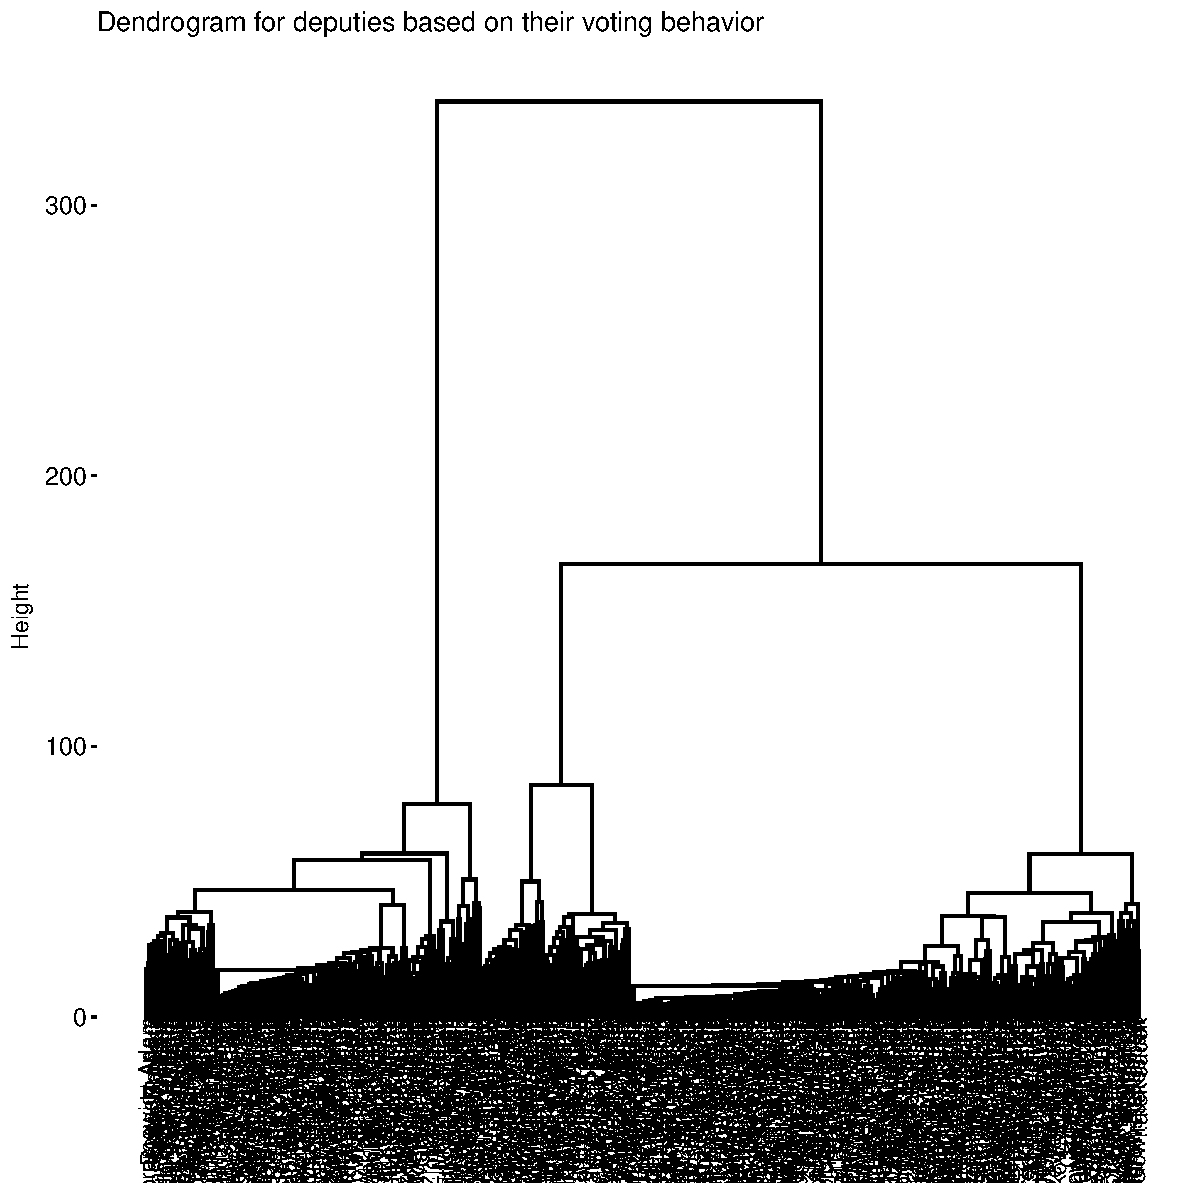
\includegraphics[width=0.8\textwidth]{ggdendro01}
  \caption{Dendrogram created with the function \texttt{get\_deputies\_dendrogram}}
  \label{figure:ggdendro}
\end{figure}


\begin{example}
> df <- votes[,c("surname_name","club")]
> df %>%
+   group_by(surname_name, club) %>%
+   summarise(n = n()) %>% 
+   arrange(-n) %>%
+   group_by(surname_name) %>%
+   top_n(1) %>%
+   as.data.frame() -> clubs
> row.names(clubs) <- clubs[,1]
> clubs$club[clubs$club == "niez."] = "cross-bencher"

> get_deputies_silhouette(mat2, clubs)
> get_deputies_mds(mat2, clubs2)

\end{example}


\section{Summary}

\CRANpkg{sejmRP} package provides easy-to-use tools to scrap and access open data from Polish Diet's webpage. Combining these tools with its further analysis and visualization
allows to build algorithms intended to reproducible statistical analysis and publication. The source code and user manual for the latest CRAN version of \CRANpkg{sejmRP} package are available at \href{https://github.com/mi2-warsaw/sejmRP}{the github site}, where can also be found the full source code of the use-cases. Despite the fact that \CRANpkg{sejmRP} package was built for Polish Diet's webpage, its infrastructure and similar analysis can be adapted to the case of other countries.

\bibliography{smuda-biecek}

\address{Piotr Smuda\\
  Faculty of Mathematics and Information Science\\
  Warsaw University of Technology\\
  Koszykowa 75, 00-662 Warsaw\\
  Poland\\}
\email{smudap@student.mini.pw.edu.pl}

\address{Przemysław Biecek\\
  Faculty of Mathematics and Information Science\\
  Warsaw University of Technology\\
  Koszykowa 75, 00-662 Warsaw\\
  Poland\\}
\email{przemyslaw.biecek@mini.pw.edu.pl}
